%\section{Anforderungen}
%\textit{In diesem Abschnitt soll die Demoanwendung vorgestellt werden, anhand dessen das Proof-of-Concept erstellt wird. Damit das Proof-of-Concept erstellt werden kann, muss die Demoanwendung die zuvor beschriebenen Probleme aufweisen, hierbei sollen die Probleme möglichst realitätsnah sein und nicht frei erfunden.}

Wie in \autoref{anf:1020} beschrieben, ist eine Demoanwendung zu erstellen, auf Basis dessen das Konzept anzuwenden ist und somit praktisch umgesetzt werden kann. Dieser Abschnitt beschäftigt sich mit der Vorstellung der Demoanwendung und der repräsentativen Aufgabe, die diese übernimmt.

In der Motivation wurde ein konkretes Problem eines Kunden der Open Knowledge genannt. Damit die Demoanwendung realistisch eine moderne Webanwendung darstellt, wird sie in Grundzügen die Webanwendung des Direktversicherers nachahmen. Bei der Webanwendung handelt es sich um eine mit Angular erstellte SPA, die den Nutzer verschiedene, teils dynamische, Formulare ausfüllen lässt und am Ende diese Daten an einen Dienst sendet und ein Ergebnis erhält, welches dargestellt wird. Während der Eingabe der Formulare werden einzelne Werte gegen Dienste validiert.

Es wurde sich dafür entschieden, dass die Webanwendung eine Bestellfunktionalität eines Obst-Webshops darstellen soll. Der Warenkorb hierfür wird anfangs dynamisch generiert und dies soll so simulieren, dass eine andere Komponente diesen erstellt hat. Der Nutzer soll seine Rechnungs- und Lieferdaten eingeben und am Ende die Bestellung ausführen können. Um das gewünschte Verhalten der Demoanwendung zu definieren, wird es im folgenden Abschnitt festgelegt.

\subsection{Verhaltensdefinition}

Mit den beiden Stakeholdern, also Christian Wansart und Stephan Müller, die beide am Projekt für den Kunden involviert sind, wurde diese Verhaltensdefinition erstellt. Diesen Ansatz der Definition der Software anhand des Verhaltens nennt man Behaviour Driven Development (BDD). Um die BDD-Definition festzuhalten wurde sie in der gängigen Gherkin \cite{Gherkin} Syntax geschrieben. Die Syntax ist natürlich zu lesen, folgend werden alle gewünschten Features der Demoanwendung in der Gherkin-Syntax aufgelistet.

\lstinputlisting[
  language = gherkin,
   caption = Demoanwendung: Gherkin Definition zum Feature \enquote{Warenkorb},
captionpos = b,
     label = lst:demoanwendung-gherkin-warenkorb
]{content/04_erstellung-poc/warenkorb-gherkin/1-warenkorb.feature}

\lstinputlisting[
  language = gherkin,
   caption = Demoanwendung: Gherkin Definition zum Feature \enquote{Rechnungsadresse},
captionpos = b,
     label = lst:demoanwendung-gherkin-rechnungsadresse
]{content/04_erstellung-poc/warenkorb-gherkin/2-rechnungsadresse.feature}

\lstinputlisting[
  language = gherkin,
   caption = Demoanwendung: Gherkin Definition zum Feature \enquote{Lieferadresse},
captionpos = b,
     label = lst:demoanwendung-gherkin-lieferadresse
]{content/04_erstellung-poc/warenkorb-gherkin/3-lieferadresse.feature}

\lstinputlisting[
  language = gherkin,
   caption = Demoanwendung: Gherkin Definition zum Feature \enquote{Zahlungsdaten},
captionpos = b,
     label = lst:demoanwendung-gherkin-zahlungsdaten
]{content/04_erstellung-poc/warenkorb-gherkin/4-zahlungsdaten.feature}

\lstinputlisting[
  language = gherkin,
   caption = Demoanwendung: Gherkin Definition zum Feature \enquote{Bestellung abschließen},
captionpos = b,
     label = lst:demoanwendung-gherkin-bestellung_abschließen
]{content/04_erstellung-poc/warenkorb-gherkin/5-bestellung_abschließen.feature}

Neben des eigentlichen User-Interfaces soll auch ein Backend teil der Demoanwendung sein. Hierfür wurde auf Basis der Verhaltensdefinition eine Architektur entworfen, die im folgenden Abschnitt näher beschrieben wird.

\subsection{Backend}

Das Backend wurde als Microservice-Architektur konzipiert und wurde ebenso wie die Webanwendung auch an das Projekt des Open Knowledge Kunden angelehnt. In \autoref{fig:demoanwendung_k8s-deployment} lässt sich die konzipierte und umgesetzte Architektur betrachten, dargestellt als Kubernetes \cite{KubernetesComponents} Deployment Diagramm. Diese Architektur wurde mit den Stakeholdern zusammen konzipiert und ähnelt dem des Direktversicherers.

Durch diese recht komplexe Architektur kann eine realitätsnahe Repräsentation erfolgen. Speziell wird bei einer solchen Architektur Tracing hilfreicher, um die Zusammenhänge zwischen den Diensten nachvollziehen zu können. Dies wird beim Einsatz und der Vorstellung der Lösung näher betrachtet.

% Die einzelnen Dienste sind als Java EE Microservices umgesetzt worden und dabei minimal gehalten worden. 

\begin{figure}[H]
	\centering
	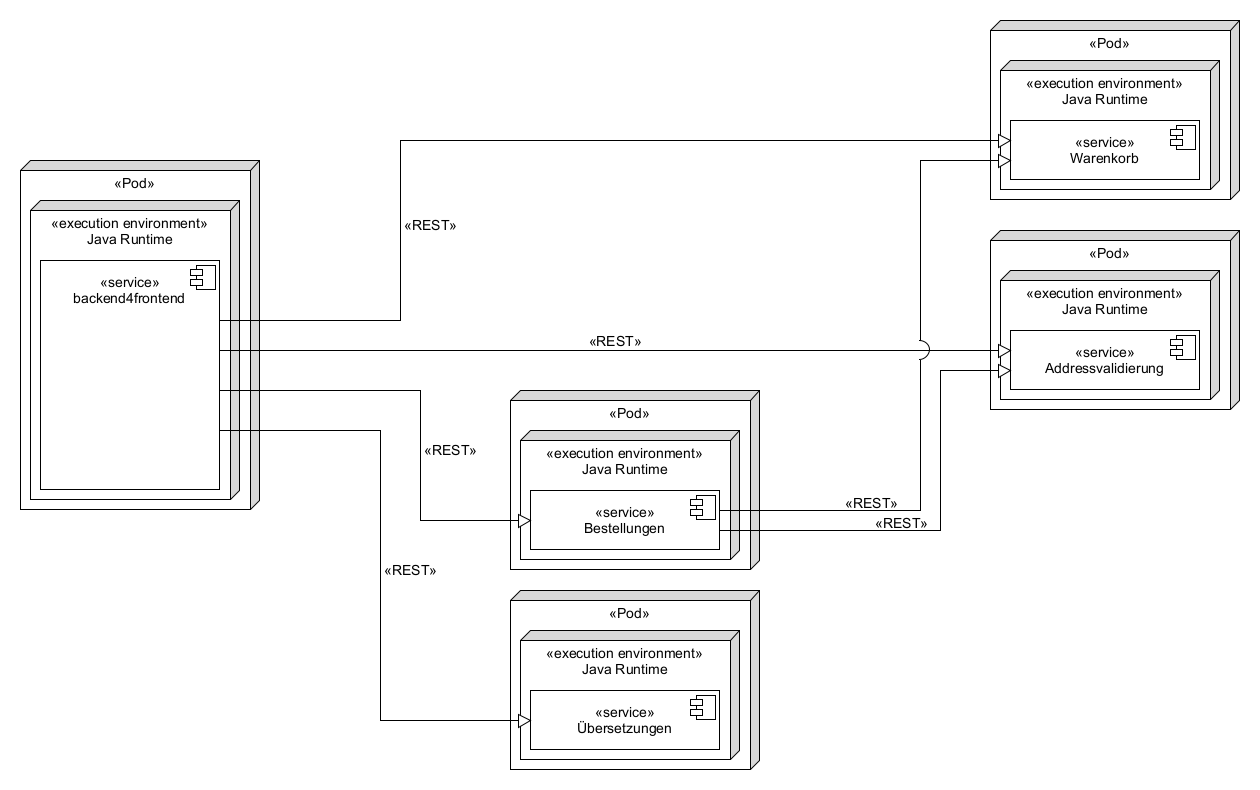
\includegraphics[width=1.0\linewidth]{img/04_erstellung-poc/demoanwendung_deployment.png}
	\caption{Demoanwendung: Deployment-Diagramm, Quelle: Eigene Darstellung}
	\label{fig:demoanwendung_deployment}
\end{figure}

\subsection{Frontend}

Das Frontend stellt das Herzstück der Demoanwendung dar und wurde auf Basis der Verhaltensdefinition erstellt. Wie beim Direktversicherer wurde es mit Angular erstellt und als zustandsreiche SPA umgesetzt. Genauere Implementierungsdetails werden jedoch nicht behandelt, außer sie sind relevant für die Lösung oder die Lösungsüberprüfung.

Das Frontend sowie das Backend wurden mit einigen Fehlern implementiert. Hintergrund ist, dass bei der Betrachtung der Lösung solche Fehler notwendig sind, um diese zu bewerten. Diese Fehler werden näher im nachfolgenden \autoref{subsec:fehlerszenarien} betrachtet.

Die einzelnen Features der Verhaltensdefinition wurden als Seiten umgesetzt und das Layout verknüpft diese Seiten in einem blätternden Format, bei dem man vor- und zurückspringen kann. Dies kann in den folgenden 6 Abbildungen betrachtet werden.

\begin{figure}[H]
	\centering
	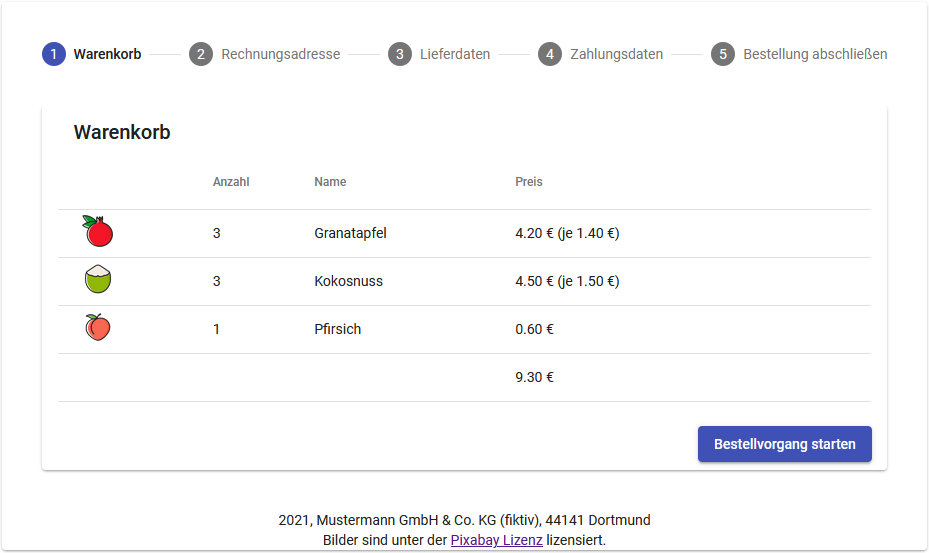
\includegraphics[width=0.75\linewidth]{img/04_erstellung-poc/demoanwendung_vorstellung_01-warenkorb.png}
	\caption{Demoanwendung: Startseite \enquote{Warenkorb}}
	\label{fig:demoanwendung_vorstellung_01-warenkorb}
\end{figure}

\begin{figure}[H]
	\centering
	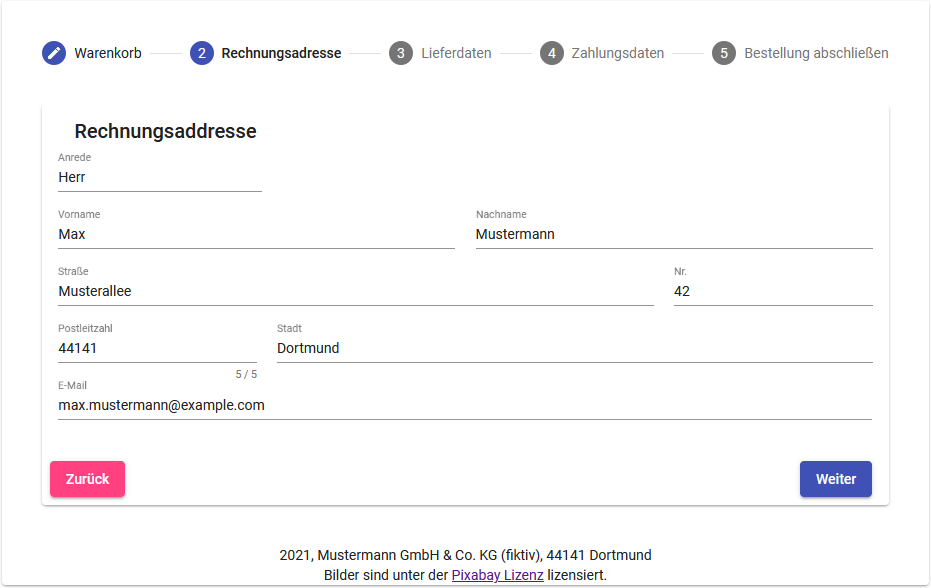
\includegraphics[width=0.75\linewidth]{img/04_erstellung-poc/demoanwendung_vorstellung_02-rechnungsadresse.png}
	\caption{Demoanwendung: Seite \enquote{Rechnungsadresse}}
	\label{fig:demoanwendung_vorstellung_02-rechnungsadresse}
\end{figure}

\begin{figure}[H]
	\centering
	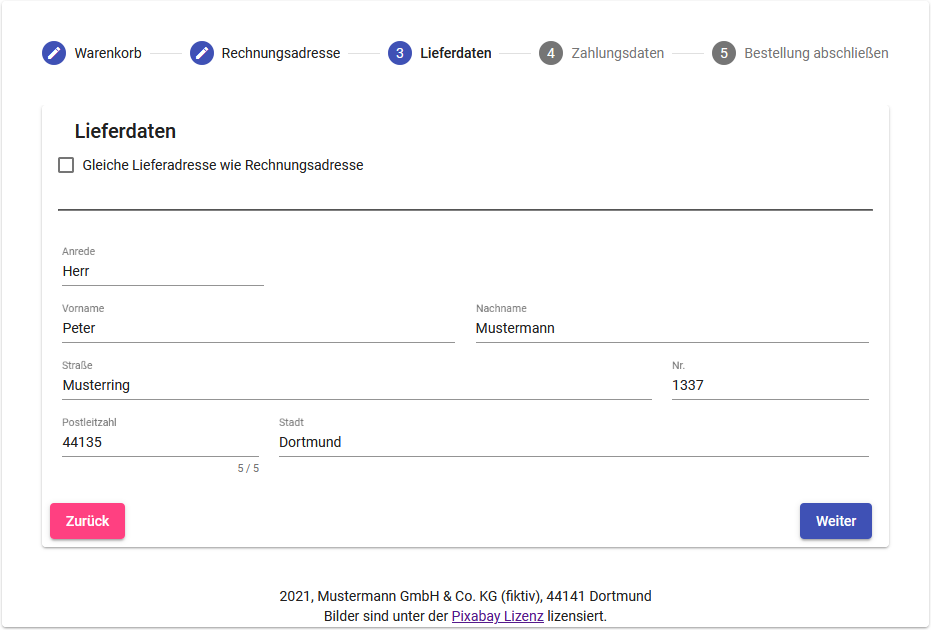
\includegraphics[width=0.75\linewidth]{img/04_erstellung-poc/demoanwendung_vorstellung_03-lieferdaten.png}
	\caption{Demoanwendung: Seite \enquote{Lieferdaten}}
	\label{fig:demoanwendung_vorstellung_03-lieferdaten}
\end{figure}

\begin{figure}[H]
	\centering
	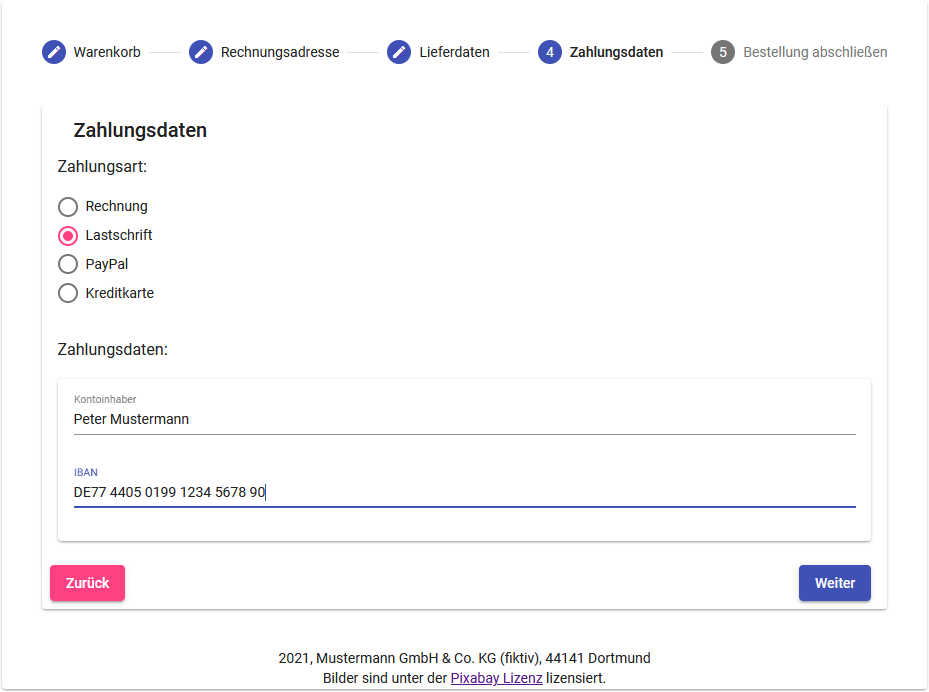
\includegraphics[width=0.75\linewidth]{img/04_erstellung-poc/demoanwendung_vorstellung_04-zahlungsdaten.png}
	\caption{Demoanwendung: Seite \enquote{Zahlungsdaten}}
	\label{fig:demoanwendung_vorstellung_04-zahlungsdaten}
\end{figure}

\begin{figure}[H]
	\centering
	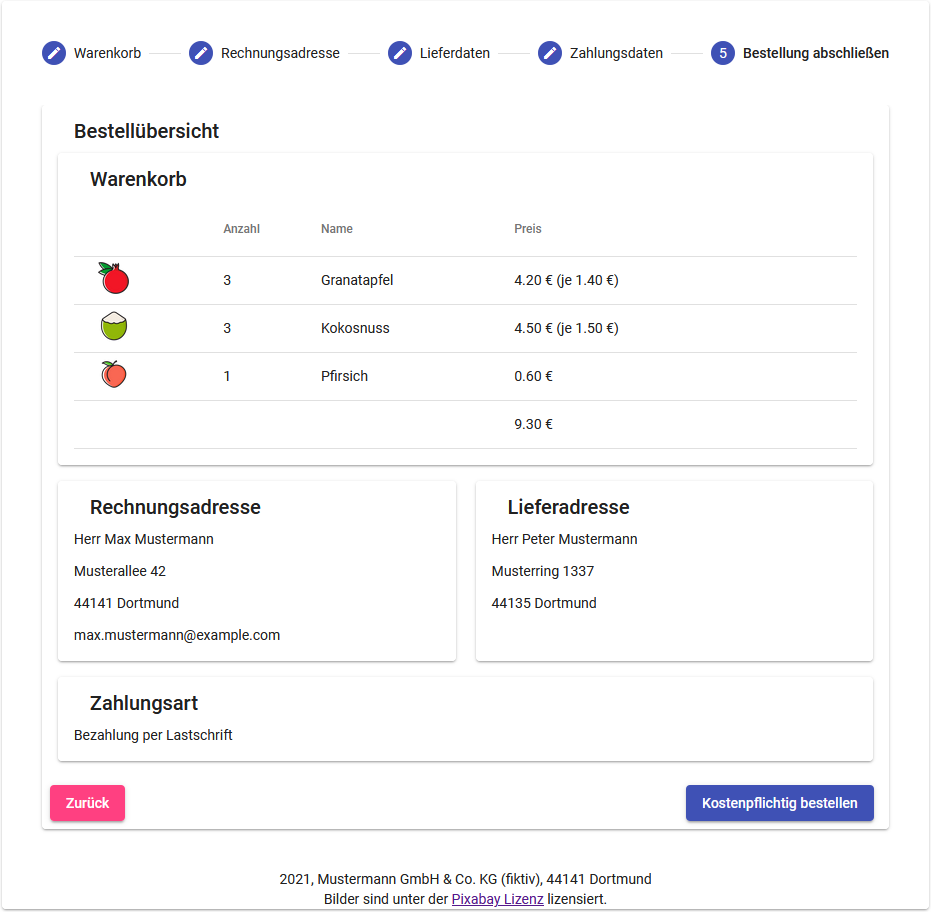
\includegraphics[width=0.75\linewidth]{img/04_erstellung-poc/demoanwendung_vorstellung_05-bestelluebersicht.png}
	\caption{Demoanwendung: Seite \enquote{Bestellübersicht}}
	\label{fig:demoanwendung_vorstellung_05-bestelluebersicht}
\end{figure}

\begin{figure}[H]
	\centering
	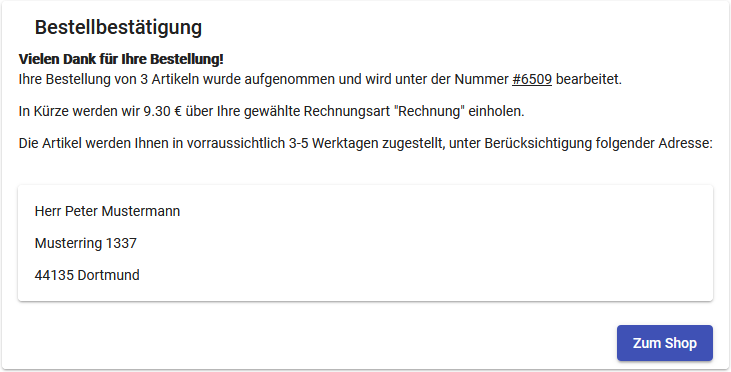
\includegraphics[width=0.75\linewidth]{img/04_erstellung-poc/demoanwendung_vorstellung_06-bestellbestaetigung.png}
	\caption{Demoanwendung: Finale Seite \enquote{Bestellbestätigung}}
	\label{fig:demoanwendung_vorstellung_06-bestellbestaetigung}
\end{figure}

\subsection{Fehlerszenarien}
\label{subsec:fehlerszenarien}

Wie zuvor erwähnt und in \autoref{anf:1020} gewünscht, besitzt die Demoanwendung einige simulierte Fehler. Diese Fehler wurden in Zusammenarbeit mit den Stakeholdern erstellt und es wurde versucht möglichst realitätsnahe oder sogar tatsächlich beim Kunden aufgetretene Probleme einzubauen.

Diese Fehler gehören unterschiedlichen Problemgruppen an, sie reichen von unerwünscht strenger Validierung, über Konfigurationsfehlern bis hin zu ineffizienter Datenverarbeitung. Sie werden mit Fehlerszenarien beschrieben, aus der Sicht eines Projektteams, welches die Szenarien berichtet bekommen oder selbst notiert hat.

\subsubsection{\enquote{Keine Übersetzungen}}

\begin{wrapfigure}[6]{r}{0.33\textwidth}
\centering
\vspace{-\baselineskip}
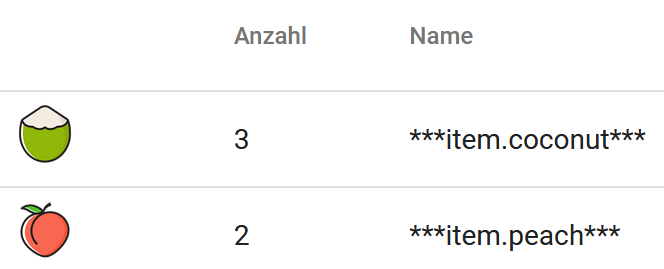
\includegraphics[width=\linewidth]{img/04_erstellung-poc/demoanwendung_fehlerszenario-uebersetzungen}
\caption{Fehlende Texte}
\label{fig:demoanwendung_fehlerszenario-uebersetzungen}
\end{wrapfigure}

- Problem: Nutzer berichten, dass manchmal die Webanwendung beim Start keine Artikeltexte anzeigt (vgl \autoref{fig:demoanwendung_fehlerszenario-uebersetzungen}).

- Ursache: Die Pods, die den Übersetzungsdienst enthalten werden repliziert bereitgestellt. Einer der Pods hat eine defekte Konfiguration, dieser ist in \autoref{fig:demoanwendung_k8s-deployment} visuell hervorgehoben. Wird man durch den LoadBalancer mit diesem Pod verbunden tritt das Fehlverhalten auf. Dies ist eine Nachstellung eines tatsächlichen Problems beim Kunden.

\subsubsection{\enquote{Gültige Straßen sind ungültig}}

- Problem: Nutzer berichten, dass Ihr Straßenname nicht eingeben werden kann. Beispielsweise die Eingabe \enquote{Ährenweg} führt zu einem Fehler.

- Ursache: Der Adressvalidierungsdienst validiert Straßen mit dem RegEx \texttt{[a-zA-Z\textbackslash,\textbackslash-\textbackslash ]+}, welches keine gängigen Sonderzeichen (ä ,ö ,ü, ß) erlaubt.

\subsubsection{\enquote{Gültige Hausnummern sind ungültig}}

- Problem: Nutzer berichten, dass Hausnummern, die nicht nur aus Zahlen bestehen, zum Fehler führen.

- Ursache: Der Adressvalidierungsdienst validiert Hausnummern als Zahl und schlägt im o. g. Fall in der Konvertierung fehl.

\subsubsection{\enquote{Gültige Städte sind ungültig}}

- Problem: Nutzer aus Gießen berichten, dass Sie das Formular zur Rechnungsadresse nicht ausfüllen können

- Ursache: Der Adressvalidierungsdienst meldet die Stadt \enquote{Gießen} als ungültig, weil sie nicht in der lokalen Tabelle vorhanden ist.

\subsubsection{\enquote{Ungültige Adressen sind gültig}}

- Problem: Nutzer können in den Lieferdaten ungültige Eingaben tätigen und absenden, bei der Bestellaufgabe kommt es zu einem Fehler.

- Ursache: Das Frontend überprüft lediglich die Rechnungsadresse, aber nicht die Lieferadresse

\subsubsection{\enquote{Vor- und Nachnamen werden abgeschnitten}}

- Problem: Nutzer berichten, dass in der Bestellbestätigung Ihre Vor- und Nachnamen abgeschnitten dargestellt werden.

- Ursache: Der Bestelldienst begrenzt den Vor- sowie den Nachnamen auf 20 Zeichen.

\subsubsection{\enquote{Falsche Zahlungsart}}

- Problem: Nutzer berichten, dass in der Bestellbestätigung die falsche Zahlungsart angezeigt wird. In der Bestellübersicht wurde jedoch die korrekte Zahlungsart angezeigt.

- Ursache: Das Frontend sendet alle Formulardaten an Bestelldienst, dieser nimmt aber an, dass alle nicht ausgewählten Formulare \texttt{null} sind.

\subsubsection{\enquote{Lange Verarbeitung}}

- Problem: Beim Absenden des Formulars auf der Seite \enquote{Warenkorb} kommt es zu einer unerwünschten Wartezeit (von min. 6-10s).

- Ursache: Dies ist eine simulierte Wartezeit im Frontend je nach Anzahl der Positionen (2s pro Position), um eine ineffiziente Verarbeitung nachzuahmen.

\subsection{Repräsentation}

Eine wichtige Eigenschaft der Demoanwendung sollte sein, dass sie repräsentativ für das Kundenprojekt und im Allgemeineren auch für SPAs ist. Durch den groben Aufbau der Demoanwendung, also einer zustandsreichen und größtenteils clientbasierten SPA, stellt die Demoanwendung eine moderne Webanwendung dar. Auch die Verwendung von Angular ist repräsentativ, denn Angular ist eines der meist verwendeten Frontend-Frameworks \cite{TheStateOfJavaScript2020}.

Weiterhin ist durch die nicht simple Backend-Architektur auch eine realitätsnähere Infrastruktur gegeben. Die Microservice-orientierte Architektur stellt zudem einen modernen Ansatz dar \cite{MicroserviceArchitecture}.

Dennoch muss gesagt werden, dass die Demoanwendung eine sehr vereinfachte Form einer modernen Webanwendung darstellt. Viel spezifischer in der Implementierung kann die Webanwendung jedoch auch nicht erstellt werden, da so die Übertragbarkeit zu anderen Projekten verloren ginge.

Nun da die Demoanwendung beschrieben ist, wird das Konzept erstellt, welches letztendlich auf die Demoanwendung anzuwenden ist. Das Konzept selber ist jedoch losgelöst von der Demoanwendung zu verstehen.